\documentclass[border=0pt,10pt]{standalone}
\usepackage[T1]{fontenc}
\usepackage{lmodern}
\usepackage{pgfplots}
\pgfplotsset{compat=1.17}
\usepgfplotslibrary{groupplots}
\usepackage{xcolor}
\definecolor{oi-blue}{HTML}{0072B2}
\definecolor{oi-vermillion}{HTML}{D55E00}
\definecolor{oi-green}{HTML}{009E73}
\definecolor{oi-purple}{HTML}{CC79A7}
\definecolor{oi-black}{HTML}{000000}
% semantic_sha256: bd2a953e6fdeba82f892112e77e569b479863bd0d1672a21f119ca1f80c333bc
\begin{document}
\begin{minipage}{181.86mm}
\centering
{\bfseries\fontsize{10}{12}\selectfont PP-U-SG | D0-M | final\_refit}\\[2mm]
{\fontsize{8}{10}\selectfont planned=780, monitored=780, missing-history=0, status=complete\_history\_coverage}\\[3mm]
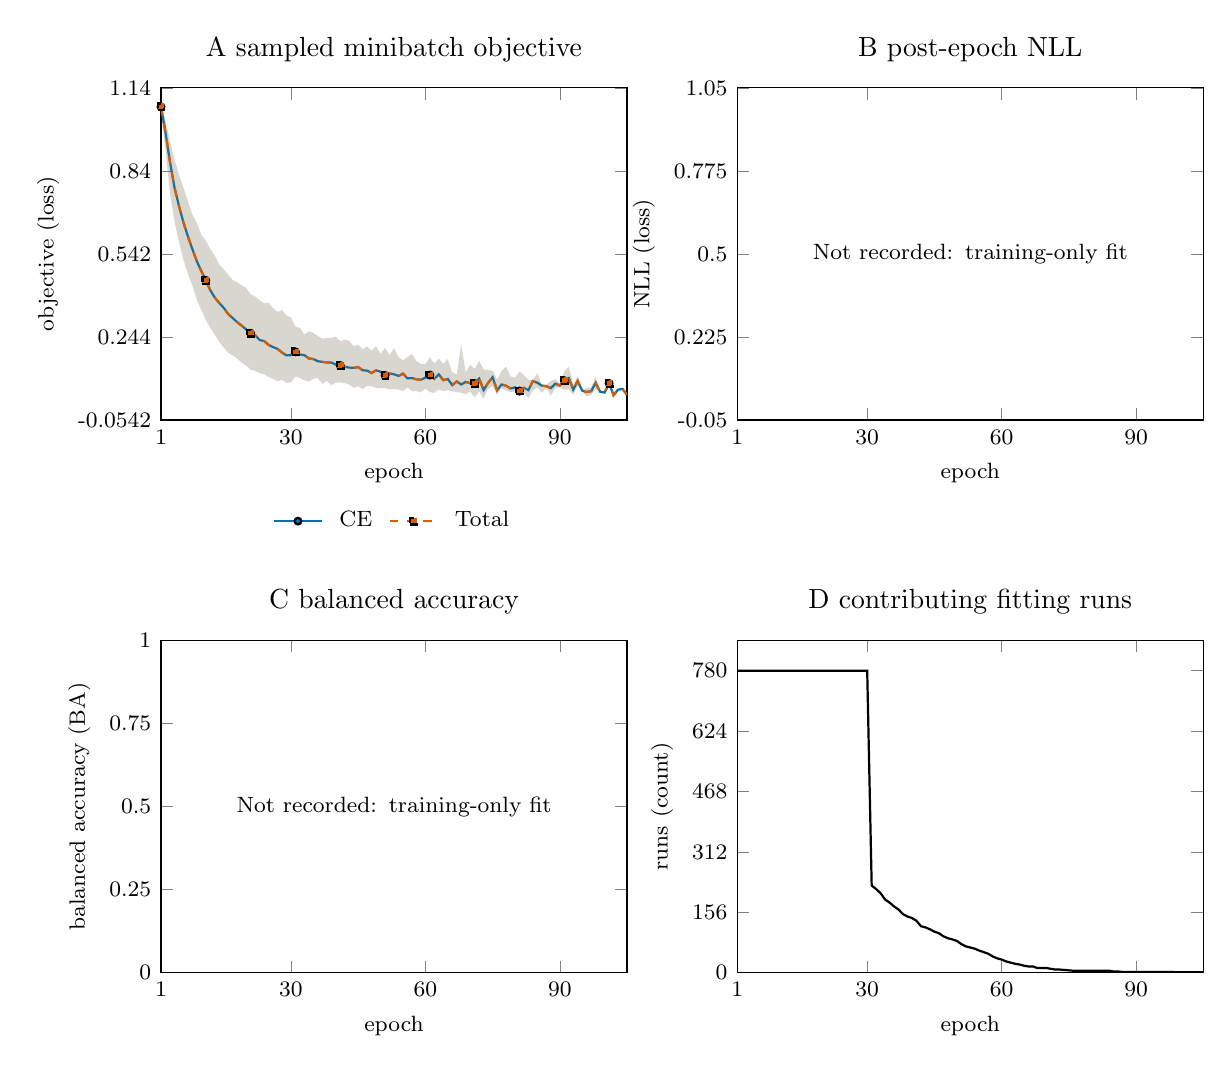
\begin{tikzpicture}
\begin{groupplot}[group style={group size=2 by 2, horizontal sep=14mm, vertical sep=28mm}]
\nextgroupplot[width=75mm, height=58mm, title={A sampled minibatch objective}, xlabel={epoch}, ylabel={objective (loss)}, xmin=1, xmax=105, xtick={1,30,60,90}, ymin=-0.05422497615218163, ymax=1.1387244991958141, ytick={-0.05422497615218163,0.24401239268481728,0.54224976152181625,0.84048713035881517,1.1387244991958141}, yticklabels={-0.0542,0.244,0.542,0.84,1.14}, tick label style={font=\fontsize{8}{9}\selectfont, text=black}, label style={font=\fontsize{8}{9}\selectfont, text=black}, title style={font=\fontsize{10}{11}\selectfont, text=black}, legend style={at={(0.5,-0.24)},anchor=north,draw=none,fill=none,font=\fontsize{8}{9}\selectfont,row sep=1pt,column sep=4pt,legend columns=2}]
\addplot[fill=oi-blue,opacity=0.15,draw=none,forget plot] coordinates {(1,1.0512959480285644) (2,0.91668377220630648) (3,0.76257309764623638) (4,0.66011179685592647) (5,0.58597203046083446) (6,0.5221566922962666) (7,0.47234791219234468) (8,0.42891090959310535) (9,0.37721257880330084) (10,0.34130256734788417) (11,0.30586655139923097) (12,0.27687166407704356) (13,0.25204671788960697) (14,0.2265702947974205) (15,0.20652695186436176) (16,0.18719653738662601) (17,0.17784166354686021) (18,0.16661112364381553) (19,0.15212433282285928) (20,0.14117223881185054) (21,0.12656692564487457) (22,0.12299704551696777) (23,0.11401003114879131) (24,0.1105278273113072) (25,0.10032732207328082) (26,0.093452092725783587) (27,0.08538047487381846) (28,0.090233844146132475) (29,0.079356793221086269) (30,0.081269575492478915) (31,0.10232859887182713) (32,0.097027512965723872) (33,0.088341950252652165) (34,0.083253613486886022) (35,0.093544822186231613) (36,0.09694623202085495) (37,0.076007612235844138) (38,0.085994997527450323) (39,0.071040710061788553) (40,0.080321761779487133) (41,0.08077046815305948) (42,0.078855439089238644) (43,0.07306578457355499) (44,0.06182787218131125) (45,0.06728303013369441) (46,0.056858521513640882) (47,0.068649454694241288) (48,0.067192672379314894) (49,0.061856670770794153) (50,0.060269905580207707) (51,0.059926671534776689) (52,0.057009013200877236) (53,0.056753176171332596) (54,0.05539960919413716) (55,0.050286545418202884) (56,0.062541754171252253) (57,0.049874998675659303) (58,0.050095784850418573) (59,0.044646379724144938) (60,0.059014444472268224) (61,0.045971073256805536) (62,0.043503158609382808) (63,0.056164538953453302) (64,0.049560308456420898) (65,0.053119749529287219) (66,0.049456838634796441) (67,0.046076310856733471) (68,0.044302969099953772) (69,0.038419535406865178) (70,0.048090389103163031) (71,0.026761484821327029) (72,0.04899098942987621) (73,0.022492425120435654) (74,0.057343708723783492) (75,0.067705777008086443) (76,0.036960410187020898) (77,0.060214263014495374) (78,0.051971269864588977) (79,0.046009955450426784) (80,0.04927555110771209) (81,0.029486968531273305) (82,0.042113219841849056) (83,0.025159572996199132) (84,0.052557514701038602) (85,0.06267272587865591) (86,0.043040063232183456) (87,0.061741313117090614) (88,0.033992804819718003) (89,0.060856485704425721) (90,0.063331194082275027) (91,0.054490136064123361) (92,0.056773251172853631) (93,0.036738717410480605) (94,0.069157081004232165) (95,0.050780650769593191) (96,0.031287773582153025) (97,0.036081605171784756) (98,0.057016307691810653) (99,0.047486455179750919) (100,0.044546981720486656) (101,0.077551621943712234) (102,0.034833961399272084) (103,0.055099545978009701) (104,0.0573059186572209) (105,0.036518165841698647) (105,0.036518165841698647) (104,0.0573059186572209) (103,0.055099545978009701) (102,0.034833961399272084) (101,0.077551621943712234) (100,0.044546981720486656) (99,0.047486455179750919) (98,0.10121532154153101) (97,0.063242674758657816) (96,0.061133505473844704) (95,0.051962455018656331) (94,0.1028461798094213) (93,0.073224775021662941) (92,0.13637320596608332) (91,0.11993222291348501) (90,0.076187970722094184) (89,0.092077304294798518) (88,0.086504338541999459) (87,0.072689766495022928) (86,0.069686296954751009) (85,0.11391774173825979) (84,0.09063819954171777) (83,0.088792064599692827) (82,0.10725575666874648) (81,0.11978015881031753) (80,0.097939110919833178) (79,0.10238081384450197) (78,0.13746435567736626) (77,0.12197827696800233) (76,0.091403187066316602) (75,0.12323369923979044) (74,0.12518276087939739) (73,0.12755250371992588) (72,0.15738178351894022) (71,0.12946752468124031) (70,0.14505736585706475) (69,0.11629952341318131) (68,0.21614793501794341) (67,0.10896105878055096) (66,0.11768315965309739) (65,0.16434361059218647) (64,0.14790282677859068) (63,0.16628933697938919) (62,0.1483443807810545) (61,0.17045976817607877) (60,0.14689259063452481) (59,0.14758711010217665) (58,0.15693656820803881) (57,0.18340163566172124) (56,0.17127359211444856) (55,0.16050870548933743) (54,0.17140335347503424) (53,0.20306920111179355) (52,0.17875957321375607) (51,0.20499195344746116) (50,0.18287490736693143) (49,0.21059209853410721) (48,0.19477516971528533) (47,0.20965019166469578) (46,0.19999100100249056) (45,0.2164620216935873) (44,0.21012939196079969) (43,0.22964745461940766) (42,0.23437175806611779) (41,0.22920815050601961) (40,0.24506133422255516) (39,0.24113530740141867) (38,0.2404327504336834) (37,0.23809746429324155) (36,0.24735245853662491) (35,0.25877150520682335) (34,0.26494134590029716) (33,0.25219357386231417) (32,0.27691804245114326) (31,0.28047443181276321) (30,0.31469321884214879) (29,0.32102550193667417) (28,0.34114891812205317) (27,0.33387486711144448) (26,0.34756305366754536) (25,0.36672985069453717) (24,0.36444712728261947) (23,0.37656129710376263) (22,0.38956456780433657) (21,0.39697445631027228) (20,0.42052740976214409) (19,0.42897246479988099) (18,0.44096185639500624) (17,0.44834798872470855) (16,0.46719699054956443) (15,0.48690090030431749) (14,0.50371311306953426) (13,0.53623696863651282) (12,0.56001735478639614) (11,0.58921989649534223) (10,0.6106274917721749) (9,0.65389603227376936) (8,0.68311911970376971) (7,0.73045274466276167) (6,0.7809568256139755) (5,0.82658913135528567) (4,0.8819209828972816) (3,0.94731752425432203) (2,1.0213720738887786) (1,1.0844995230436325)};
\addplot[color=oi-blue, mark=*, mark options={draw=black}, mark repeat=10, mark size=1.2pt, solid, line width=0.8pt] coordinates {(1,1.0709725767374039) (2,0.97927015274763107) (3,0.87320918589830399) (4,0.78189640492200851) (5,0.71515266597270966) (6,0.65592288970947266) (7,0.6056128516793251) (8,0.55979184061288834) (9,0.51594500988721848) (10,0.4808042086660862) (11,0.44760721176862717) (12,0.41184680536389351) (13,0.38574394956231117) (14,0.36616415902972221) (15,0.34872003272175789) (16,0.32637188024818897) (17,0.31205031462013721) (18,0.29730271548032761) (19,0.28482199087738991) (20,0.27133933082222939) (21,0.25751230679452419) (22,0.25101026706397533) (23,0.23320849426090717) (24,0.22950541973114014) (25,0.21593273896723986) (26,0.20766223967075348) (27,0.20148482453078032) (28,0.18822784908115864) (29,0.17795307096093893) (30,0.17864655703306198) (31,0.1906123012304306) (32,0.18111907318234444) (33,0.1786632239818573) (34,0.16694428026676178) (35,0.16472502239048481) (36,0.15707386168651283) (37,0.15464429929852486) (38,0.15247022546827793) (39,0.15229650586843491) (40,0.14526586607098579) (41,0.14183157030493021) (42,0.1369376580696553) (43,0.13410707376897335) (44,0.13336192583665252) (45,0.13590379897505045) (46,0.1245476370677352) (47,0.12322895601391792) (48,0.11457788944244385) (49,0.12423727090936154) (50,0.11947720032185316) (51,0.10605236422270536) (52,0.11341761145740747) (53,0.1101127490401268) (54,0.10425673797726631) (55,0.11217562388628721) (56,0.095508875325322151) (57,0.09658132866024971) (58,0.09198429062962532) (59,0.090422585606575012) (60,0.098002409562468529) (61,0.10729462932795286) (62,0.093785893172025681) (63,0.10973068326711655) (64,0.088917848654091358) (65,0.093397155404090881) (66,0.07101684994995594) (67,0.084535720525309443) (68,0.07332951424177736) (69,0.082712679752148688) (70,0.078150933608412743) (71,0.07722722040489316) (72,0.094692562008276582) (73,0.053422297351062298) (74,0.079331754008308053) (75,0.099499598145484924) (76,0.052580898627638817) (77,0.073474489618092775) (78,0.069200647529214621) (79,0.059010124299675226) (80,0.063018740154802799) (81,0.050003307638689876) (82,0.061407402623444796) (83,0.053270900971256196) (84,0.085590420290827751) (85,0.079552897252142429) (86,0.069222709164023399) (87,0.067215539806056768) (88,0.060248571680858731) (89,0.076466894999612123) (90,0.069759582402184606) (91,0.087211179488804191) (92,0.096573228569468483) (93,0.05498174621607177) (94,0.086001630406826735) (95,0.051371552894124761) (96,0.046210639527998865) (97,0.049662139965221286) (98,0.079115814616670832) (99,0.047486455179750919) (100,0.044546981720486656) (101,0.077551621943712234) (102,0.034833961399272084) (103,0.055099545978009701) (104,0.0573059186572209) (105,0.036518165841698647)};
\addlegendentry{CE}
\addplot[fill=oi-vermillion,opacity=0.15,draw=none,forget plot] coordinates {(1,1.0512959480285644) (2,0.91668377220630648) (3,0.76257309764623638) (4,0.66011179685592647) (5,0.58597203046083446) (6,0.5221566922962666) (7,0.47234791219234468) (8,0.42891090959310535) (9,0.37721257880330084) (10,0.34130256734788417) (11,0.30586655139923097) (12,0.27687166407704356) (13,0.25204671788960697) (14,0.2265702947974205) (15,0.20652695186436176) (16,0.18719653738662601) (17,0.17784166354686021) (18,0.16661112364381553) (19,0.15212433282285928) (20,0.14117223881185054) (21,0.12656692564487457) (22,0.12299704551696777) (23,0.11401003114879131) (24,0.1105278273113072) (25,0.10032732207328082) (26,0.093452092725783587) (27,0.08538047487381846) (28,0.090233844146132475) (29,0.079356793221086269) (30,0.081269575492478915) (31,0.10232859887182713) (32,0.097027512965723872) (33,0.088341950252652165) (34,0.083253613486886022) (35,0.093544822186231613) (36,0.09694623202085495) (37,0.076007612235844138) (38,0.085994997527450323) (39,0.071040710061788553) (40,0.080321761779487133) (41,0.08077046815305948) (42,0.078855439089238644) (43,0.07306578457355499) (44,0.06182787218131125) (45,0.06728303013369441) (46,0.056858521513640882) (47,0.068649454694241288) (48,0.067192672379314894) (49,0.061856670770794153) (50,0.060269905580207707) (51,0.059926671534776689) (52,0.057009013200877236) (53,0.056753176171332596) (54,0.05539960919413716) (55,0.050286545418202884) (56,0.062541754171252253) (57,0.049874998675659303) (58,0.050095784850418573) (59,0.044646379724144938) (60,0.059014444472268224) (61,0.045971073256805536) (62,0.043503158609382808) (63,0.056164538953453302) (64,0.049560308456420898) (65,0.053119749529287219) (66,0.049456838634796441) (67,0.046076310856733471) (68,0.044302969099953772) (69,0.038419535406865178) (70,0.048090389103163031) (71,0.026761484821327029) (72,0.04899098942987621) (73,0.022492425120435654) (74,0.057343708723783492) (75,0.067705777008086443) (76,0.036960410187020898) (77,0.060214263014495374) (78,0.051971269864588977) (79,0.046009955450426784) (80,0.04927555110771209) (81,0.029486968531273305) (82,0.042113219841849056) (83,0.025159572996199132) (84,0.052557514701038602) (85,0.06267272587865591) (86,0.043040063232183456) (87,0.061741313117090614) (88,0.033992804819718003) (89,0.060856485704425721) (90,0.063331194082275027) (91,0.054490136064123361) (92,0.056773251172853631) (93,0.036738717410480605) (94,0.069157081004232165) (95,0.050780650769593191) (96,0.031287773582153025) (97,0.036081605171784756) (98,0.057016307691810653) (99,0.047486455179750919) (100,0.044546981720486656) (101,0.077551621943712234) (102,0.034833961399272084) (103,0.055099545978009701) (104,0.0573059186572209) (105,0.036518165841698647) (105,0.036518165841698647) (104,0.0573059186572209) (103,0.055099545978009701) (102,0.034833961399272084) (101,0.077551621943712234) (100,0.044546981720486656) (99,0.047486455179750919) (98,0.10121532154153101) (97,0.063242674758657816) (96,0.061133505473844704) (95,0.051962455018656331) (94,0.1028461798094213) (93,0.073224775021662941) (92,0.13637320596608332) (91,0.11993222291348501) (90,0.076187970722094184) (89,0.092077304294798518) (88,0.086504338541999459) (87,0.072689766495022928) (86,0.069686296954751009) (85,0.11391774173825979) (84,0.09063819954171777) (83,0.088792064599692827) (82,0.10725575666874648) (81,0.11978015881031753) (80,0.097939110919833178) (79,0.10238081384450197) (78,0.13746435567736626) (77,0.12197827696800233) (76,0.091403187066316602) (75,0.12323369923979044) (74,0.12518276087939739) (73,0.12755250371992588) (72,0.15738178351894022) (71,0.12946752468124031) (70,0.14505736585706475) (69,0.11629952341318131) (68,0.21614793501794341) (67,0.10896105878055096) (66,0.11768315965309739) (65,0.16434361059218647) (64,0.14790282677859068) (63,0.16628933697938919) (62,0.1483443807810545) (61,0.17045976817607877) (60,0.14689259063452481) (59,0.14758711010217665) (58,0.15693656820803881) (57,0.18340163566172124) (56,0.17127359211444856) (55,0.16050870548933743) (54,0.17140335347503424) (53,0.20306920111179355) (52,0.17875957321375607) (51,0.20499195344746116) (50,0.18287490736693143) (49,0.21059209853410721) (48,0.19477516971528533) (47,0.20965019166469578) (46,0.19999100100249056) (45,0.2164620216935873) (44,0.21012939196079969) (43,0.22964745461940766) (42,0.23437175806611779) (41,0.22920815050601961) (40,0.24506133422255516) (39,0.24113530740141867) (38,0.2404327504336834) (37,0.23809746429324155) (36,0.24735245853662491) (35,0.25877150520682335) (34,0.26494134590029716) (33,0.25219357386231417) (32,0.27691804245114326) (31,0.28047443181276321) (30,0.31469321884214879) (29,0.32102550193667417) (28,0.34114891812205317) (27,0.33387486711144448) (26,0.34756305366754536) (25,0.36672985069453717) (24,0.36444712728261947) (23,0.37656129710376263) (22,0.38956456780433657) (21,0.39697445631027228) (20,0.42052740976214409) (19,0.42897246479988099) (18,0.44096185639500624) (17,0.44834798872470855) (16,0.46719699054956443) (15,0.48690090030431749) (14,0.50371311306953426) (13,0.53623696863651282) (12,0.56001735478639614) (11,0.58921989649534223) (10,0.6106274917721749) (9,0.65389603227376936) (8,0.68311911970376971) (7,0.73045274466276167) (6,0.7809568256139755) (5,0.82658913135528567) (4,0.8819209828972816) (3,0.94731752425432203) (2,1.0213720738887786) (1,1.0844995230436325)};
\addplot[color=oi-vermillion, mark=square*, mark options={draw=black}, mark repeat=10, mark size=1.2pt, dashed, line width=0.8pt] coordinates {(1,1.0709725767374039) (2,0.97927015274763107) (3,0.87320918589830399) (4,0.78189640492200851) (5,0.71515266597270966) (6,0.65592288970947266) (7,0.6056128516793251) (8,0.55979184061288834) (9,0.51594500988721848) (10,0.4808042086660862) (11,0.44760721176862717) (12,0.41184680536389351) (13,0.38574394956231117) (14,0.36616415902972221) (15,0.34872003272175789) (16,0.32637188024818897) (17,0.31205031462013721) (18,0.29730271548032761) (19,0.28482199087738991) (20,0.27133933082222939) (21,0.25751230679452419) (22,0.25101026706397533) (23,0.23320849426090717) (24,0.22950541973114014) (25,0.21593273896723986) (26,0.20766223967075348) (27,0.20148482453078032) (28,0.18822784908115864) (29,0.17795307096093893) (30,0.17864655703306198) (31,0.1906123012304306) (32,0.18111907318234444) (33,0.1786632239818573) (34,0.16694428026676178) (35,0.16472502239048481) (36,0.15707386168651283) (37,0.15464429929852486) (38,0.15247022546827793) (39,0.15229650586843491) (40,0.14526586607098579) (41,0.14183157030493021) (42,0.1369376580696553) (43,0.13410707376897335) (44,0.13336192583665252) (45,0.13590379897505045) (46,0.1245476370677352) (47,0.12322895601391792) (48,0.11457788944244385) (49,0.12423727090936154) (50,0.11947720032185316) (51,0.10605236422270536) (52,0.11341761145740747) (53,0.1101127490401268) (54,0.10425673797726631) (55,0.11217562388628721) (56,0.095508875325322151) (57,0.09658132866024971) (58,0.09198429062962532) (59,0.090422585606575012) (60,0.098002409562468529) (61,0.10729462932795286) (62,0.093785893172025681) (63,0.10973068326711655) (64,0.088917848654091358) (65,0.093397155404090881) (66,0.07101684994995594) (67,0.084535720525309443) (68,0.07332951424177736) (69,0.082712679752148688) (70,0.078150933608412743) (71,0.07722722040489316) (72,0.094692562008276582) (73,0.053422297351062298) (74,0.079331754008308053) (75,0.099499598145484924) (76,0.052580898627638817) (77,0.073474489618092775) (78,0.069200647529214621) (79,0.059010124299675226) (80,0.063018740154802799) (81,0.050003307638689876) (82,0.061407402623444796) (83,0.053270900971256196) (84,0.085590420290827751) (85,0.079552897252142429) (86,0.069222709164023399) (87,0.067215539806056768) (88,0.060248571680858731) (89,0.076466894999612123) (90,0.069759582402184606) (91,0.087211179488804191) (92,0.096573228569468483) (93,0.05498174621607177) (94,0.086001630406826735) (95,0.051371552894124761) (96,0.046210639527998865) (97,0.049662139965221286) (98,0.079115814616670832) (99,0.047486455179750919) (100,0.044546981720486656) (101,0.077551621943712234) (102,0.034833961399272084) (103,0.055099545978009701) (104,0.0573059186572209) (105,0.036518165841698647)};
\addlegendentry{Total}
\nextgroupplot[width=75mm, height=58mm, title={B post-epoch NLL}, xlabel={epoch}, ylabel={NLL (loss)}, xmin=1, xmax=105, xtick={1,30,60,90}, ymin=-0.050000000000000003, ymax=1.05, ytick={-0.050000000000000003,0.22500000000000003,0.5,0.77500000000000002,1.05}, yticklabels={-0.05,0.225,0.5,0.775,1.05}, tick label style={font=\fontsize{8}{9}\selectfont, text=black}, label style={font=\fontsize{8}{9}\selectfont, text=black}, title style={font=\fontsize{10}{11}\selectfont, text=black}]
\node[align=center, text width=55mm, font=\fontsize{8}{9}\selectfont] at (axis cs:53,0.5) {Not recorded: training-only fit};
\nextgroupplot[width=75mm, height=58mm, title={C balanced accuracy}, xlabel={epoch}, ylabel={balanced accuracy (BA)}, xmin=1, xmax=105, xtick={1,30,60,90}, ymin=0, ymax=1, ytick={0,0.25,0.5,0.75,1}, yticklabels={0,0.25,0.5,0.75,1}, tick label style={font=\fontsize{8}{9}\selectfont, text=black}, label style={font=\fontsize{8}{9}\selectfont, text=black}, title style={font=\fontsize{10}{11}\selectfont, text=black}]
\node[align=center, text width=55mm, font=\fontsize{8}{9}\selectfont] at (axis cs:53,0.5) {Not recorded: training-only fit};
\nextgroupplot[width=75mm, height=58mm, title={D contributing fitting runs}, xlabel={epoch}, ylabel={runs (count)}, xmin=1, xmax=105, xtick={1,30,60,90}, ymin=0, ymax=858.00000000000011, ytick={0,156,312,468,624,780}, yticklabels={0,156,312,468,624,780}, tick label style={font=\fontsize{8}{9}\selectfont, text=black}, label style={font=\fontsize{8}{9}\selectfont, text=black}, title style={font=\fontsize{10}{11}\selectfont, text=black}]
\addplot[color=oi-black, solid, line width=0.8pt] coordinates {(1,780) (2,780) (3,780) (4,780) (5,780) (6,780) (7,780) (8,780) (9,780) (10,780) (11,780) (12,780) (13,780) (14,780) (15,780) (16,780) (17,780) (18,780) (19,780) (20,780) (21,780) (22,780) (23,780) (24,780) (25,780) (26,780) (27,780) (28,780) (29,780) (30,780) (31,225) (32,216) (33,205) (34,189) (35,181) (36,171) (37,163) (38,151) (39,145) (40,141) (41,134) (42,120) (43,117) (44,112) (45,106) (46,102) (47,94) (48,89) (49,86) (50,82) (51,74) (52,68) (53,65) (54,62) (55,57) (56,53) (57,49) (58,42) (59,37) (60,34) (61,29) (62,26) (63,23) (64,21) (65,18) (66,16) (67,16) (68,12) (69,12) (70,12) (71,10) (72,8) (73,8) (74,7) (75,6) (76,5) (77,5) (78,5) (79,5) (80,5) (81,5) (82,5) (83,5) (84,5) (85,3) (86,3) (87,2) (88,2) (89,2) (90,2) (91,2) (92,2) (93,2) (94,2) (95,2) (96,2) (97,2) (98,2) (99,1) (100,1) (101,1) (102,1) (103,1) (104,1) (105,1)};
\end{groupplot}
\end{tikzpicture}
\par\vspace{6mm}
\begin{minipage}{175mm}
{\fontsize{8}{10}\selectfont RQ-S01 / Scope E: descriptive training diagnostics. 400-1800 cm-1 inputs: SG uses impulse replacement and Savitzky-Golay smoothing; arPLS uses impulse replacement and baseline correction; both finish with [0,1] min-max scaling. CE = chemical cross-entropy; SupCon = supervised contrastive; Paired = paired consistency; NLL = negative log-likelihood; BA = balanced accuracy. Authenticated complete monitor histories aggregated across unique fitting jobs into descriptive policy/recipe/stage curves. Curves summarize per-epoch minibatch-weighted training chemical cross-entropy and the composite total optimization objective; these sampled minibatch objectives differ from post-epoch evaluation negative log-likelihood. Auxiliary supcon/paired loss components are recipe-specific and are not directly comparable to the total objective across recipes. Validation metrics are recorded for source\_fit runs only and never substitute for a held-out test set; calibration\_model\_fit and final\_refit rows carry training-only diagnostics. Source\_fit optimization uses a 30-epoch minimum stopping threshold and a 200-epoch maximum; refit stages reuse the caller-selected duration. Curves are fitting-run-weighted descriptive summaries over correlated runs (seeds/splits). Lines show medians; 10th/90th percentiles describe variation among saved fitting runs, not confidence intervals. Only runs that reached each epoch contribute; early stopping changes the composition, and stopped runs are not carried forward. Fitting jobs are not independent chemical samples: the dataset has 598 spectra from 69 physical samples and 10 instruments. Coverage is limited to saved SG/arPLS monitor histories; historical MIN losses are not pooled or invented. A missing history is not a zero loss or proof of a failed model. These curves do not support hypothesis tests, superiority claims, model selection, or new uncertainty inference. P08 learned-method performance is reported elsewhere.}
\end{minipage}
\end{minipage}
\end{document}